\ifdefined\XeTeXrevision\else\pdfoutput=1\fi
\documentclass[11pt]{article}
\usepackage[margin=1in]{geometry}
\usepackage{graphicx}
\usepackage{booktabs}
\usepackage{amsmath}
\usepackage{amssymb}
\usepackage{caption}
\usepackage{enumitem}
\usepackage{xcolor}
\usepackage{hyperref}
\usepackage{microtype}
\hypersetup{
  colorlinks=true,
  linkcolor=blue!60!black,
  citecolor=blue!60!black,
  urlcolor=blue!60!black,
  pdftitle={Conditional LoRA Bridges for Modular Sensor Adaptation of Frozen Small Language Models},
  pdfauthor={Franci Penov},
}
\graphicspath{{figures/}}
\title{Conditional LoRA Bridges for Modular Sensor Adaptation of Frozen Small Language Models}
\author{Franci Penov \\ kortexa.ai \\ \texttt{francip@kortexa.ai}}
\date{2026-06-09}

\begin{document}
\maketitle

\begin{abstract}
We study whether frozen language models can be conditioned on external sensor streams by generating Low-Rank Adaptation (LoRA) weights at runtime. A conditional LoRA bridge maps frozen sensor-encoder features to per-input LoRA parameters that are injected into a frozen transformer without changing base model weights. On a controlled 33.6M-parameter Qwen-style language model, we evaluate dynamic bridges alongside static LoRA, shuffled-, random-, and constant-feature controls, prefix tuning, composition tests, task-aligned ranking probes, and seed-stability checks, all under one fixed-step runner. The decomposition is sharp. Measured by validation bits-per-byte, conditioning contributes nothing: a capacity-matched bridge fed one constant feature vector matches the true-feature bridge, and static LoRA beats both. Measured by task-aligned probes, conditioning is decisive: with true features the frozen model ranks the correct sensor label first 0.80 of the time on six-way IMU activities and 0.33 on fifty-way audio events, while shuffled features, random features, and the unconditioned model all sit at chance. Aggregate language-modeling metrics are therefore the wrong instrument for detecting sensor conditioning. Diversity regularization governs the central failure mode: without it, generated weights collapse toward input-independence --- and at sufficiently long training budgets this collapse erases the task-level conditioning entirely. Prefix tuning, the token-space alternative, only degrades the frozen model. These results support weight-space modulation as a viable modular interface between independently trained sensor encoders and frozen language models, with bridge compression and regularized long-horizon training as the open problems.
\end{abstract}

\section{Introduction}
Multimodal language models are often extended by joint training on paired multimodal corpora. That recipe is powerful, but it is awkward for small or local systems: every new sensor type can require a new data collection pipeline, new paired examples, and another round of model adaptation. This paper studies a narrower interface: keep the language model frozen, keep the sensor encoder frozen, and learn only a bridge that converts sensor features into LoRA weights.

The method, which we call \emph{conditional LoRA bridges}, uses a hypernetwork \cite{ha2016hypernetworks} to generate LoRA parameters \cite{hu2021lora} from sensor features. The generated low-rank matrices are injected into a frozen transformer at runtime. The mechanism is related to adapters \cite{houlsby2019adapters}, shared hypernetwork adapters \cite{mahabadi2021hyperformer}, and prefix tuning \cite{li2021prefixtuning}, but differs by conditioning weight-space updates on continuous external sensor streams rather than appending tokens or selecting a task identifier.

Contributions:
\begin{itemize}[leftmargin=*]
  \item A controlled, fully reproducible evaluation harness for conditional LoRA bridges across vision, audio, and IMU features: fixed step counts, a shared eval stream, three-seed checks, and every table and number in this manuscript rendered from a single bundled result artifact.
  \item A capacity/conditioning decomposition via controls. A constant-feature bridge isolates trainable capacity; it matches the true-feature bridge on BPB (+0.0027 vs.\ +0.0027), showing that aggregate language-modeling gains carry no evidence of sensor conditioning.
  \item Task-aligned probes that detect conditioning decisively where BPB cannot: true features lift rank-1 label accuracy to 0.80 (IMU, chance 0.17) and 0.33 (audio, chance 0.02) while every control stays at chance.
  \item A characterization of hypernetwork weight collapse: diversity regularization makes generated weights input-dependent, and at long training budgets unregularized bridges collapse to input-independence, erasing task-level conditioning (Section~\ref{sec:scaling}).
\end{itemize}

\section{Method}
\paragraph{Frozen language model.}
The base model is an eight-layer, 512-hidden-dimension Qwen-style decoder-only transformer (33.6M parameters, tied embeddings counted once) with grouped-query attention, SwiGLU feed-forward blocks, rotary position embeddings, and an 8192-token BPE vocabulary. The shipped checkpoint evaluates at 1.9654 BPB under this runner.

\paragraph{Sensor encoders.}
We use three frozen encoders: a MobileNetV3-style frame encoder plus Perceiver resampler for vision, a Conv1D audio encoder over mel spectrograms for ESC-50-style audio features, and a Conv1D IMU encoder over UCI-HAR accelerometer/gyroscope windows. The bridge consumes only encoder features; raw sensor processing remains outside the language model.

\paragraph{Bridge hypernetwork.}
For a sensor feature vector $f$, the bridge predicts a flattened LoRA vector $w = h_\theta(f)$. The vector is partitioned into LoRA matrices $(A_i, B_i)$ for each target linear layer. During a forward pass, a frozen linear layer computes
\[
  y = xW + \alpha x A_i B_i / r,
\]
where $r$ is the LoRA rank and $\alpha$ is the LoRA scale. The base weights $W$ and sensor encoder are frozen; only bridge parameters are optimized.

\paragraph{Diversity regularization.}
A bridge can minimize text loss while emitting nearly identical LoRA weights for all inputs. To measure and penalize this collapse, we add a cosine diversity term across generated weights in a batch:
\[
  \mathcal{L}_\text{div} = \frac{1}{N(N-1)} \sum_{i \ne j} \cos(w_i, w_j).
\]
Lower cosine similarity indicates more input-dependent generated weights.

\section{Experimental Setup}
The primary metric is validation bits-per-byte (BPB) on held-out text; lower BPB is better, and tables report improvement relative to the frozen baseline. Every condition is evaluated on the same fixed 32768-token validation stream, so all reported deltas are paired comparisons; the absolute BPB level would shift by roughly $\pm 0.02$ under an independent eval sample of the same size. BPB gives a stable language-modeling measurement, but it is not sufficient evidence of semantic sensor use. We therefore include shuffled-feature, random-feature, and constant-feature controls, task-aligned ranking probes, composition tests, and held-out weight-space structure probes.

The full run used rank 4, target set all, bridge learning rate 0.001, 300 benchmark training steps, 150 composition steps per brick, 600 task-probe training steps, and seeds 42, 1042, 2042. The result artifact is the summary JSON consumed by the figure and manuscript renderers.

\section{Results}
\subsection{Bridge and baseline comparison}
Table~\ref{tab:main} and Figure~\ref{fig:main} summarize BPB improvements across modalities. Static LoRA measures the gain from fixed low-rank adaptation; the constant-feature bridge is the capacity-matched control (the full hypernetwork trains, but its input never varies); random features test stochastic conditioning; shuffled features map sensor indices through a fixed derangement.

The BPB outcome is unambiguous and deliberately deflationary. Static LoRA is the best text adapter (+0.0033 mean): direct optimization beats hypernetwork-mediated optimization when only text quality matters. The conditional bridge (+0.0027) is statistically inseparable from the constant-feature control (+0.0027) --- the bridge's entire BPB gain is explained by its trainable capacity, with no measurable contribution from the sensor signal. We note that in this pipeline text batches and sensor draws are sampled independently, so there is no semantic sensor--text alignment for the shuffled control to destroy; shuffled (+0.0018) functions as a seed-noise sanity check here, and the semantically meaningful shuffled control appears in the task probes below, where features are label-paired.

\begin{table}[t]
\centering
\caption{BPB improvement relative to the frozen mini-model baseline. Positive values are better. Static LoRA consumes no sensor input, so its per-modality cells repeat the same seeded modality-independent run.}
\label{tab:main}
\begin{tabular}{lrrrr}
\toprule
Method & Audio & Vision & IMU & Mean \\
\midrule
Static LoRA & +0.0033 & +0.0033 & +0.0033 & +0.0033 \\
Conditional bridge & +0.0025 & +0.0031 & +0.0026 & +0.0027 \\
Shuffled features & +0.0030 & +0.0003 & +0.0021 & +0.0018 \\
Random features & +0.0006 & +0.0010 & +0.0001 & +0.0006 \\
Constant features & +0.0027 & +0.0023 & +0.0030 & +0.0027 \\
Prefix tuning & -0.0049 & -0.0047 & -0.0048 & -0.0048 \\
\bottomrule
\end{tabular}
\end{table}

\begin{figure}[t]
\centering
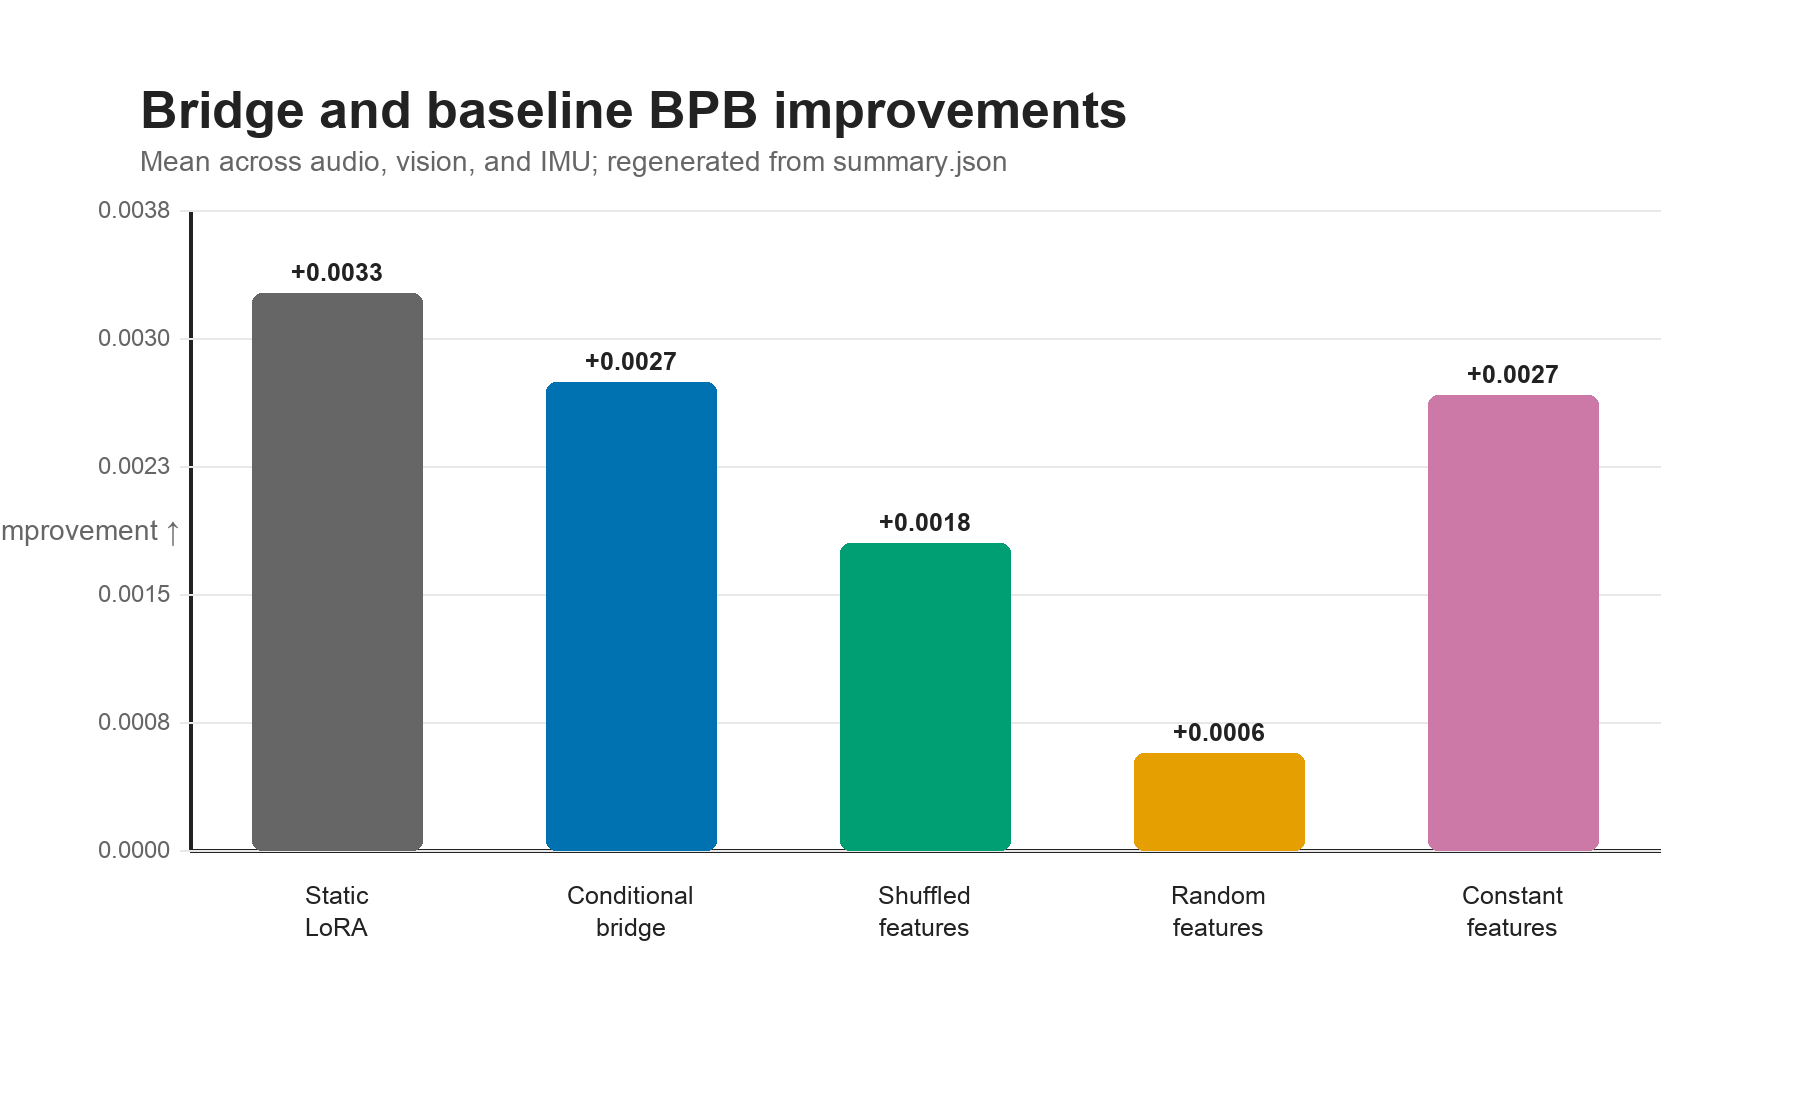
\includegraphics[width=0.82\linewidth]{paper_main_benchmark.png}
\caption{Mean BPB improvement across audio, vision, and IMU. The controls show that capacity and regularization explain part of the bridge gain.}
\label{fig:main}
\end{figure}

Prefix tuning, the token-space alternative, degrades BPB (-0.0048 mean): inserting learned continuous tokens shifts the position distribution a frozen small model was trained under, and within this budget the prefix never recovers the loss it induces, let alone improves on the baseline. The contrast with the uniformly positive weight-space rows is the practical takeaway --- for frozen small models, weight modulation is the conditioning path that does no harm.

\subsection{Feature controls}
Figure~\ref{fig:controls} restates the interpretation problem visually: true, shuffled, and constant features achieve nearly identical BPB, so BPB is measuring bridge capacity, not semantic sensor conditioning. Any claim of genuine conditioning must therefore rest on probes that are sensitive to per-input behavior --- the task-aligned probes below and the weight-space structure analysis of Section~\ref{sec:diversity}.

\begin{figure}[t]
\centering
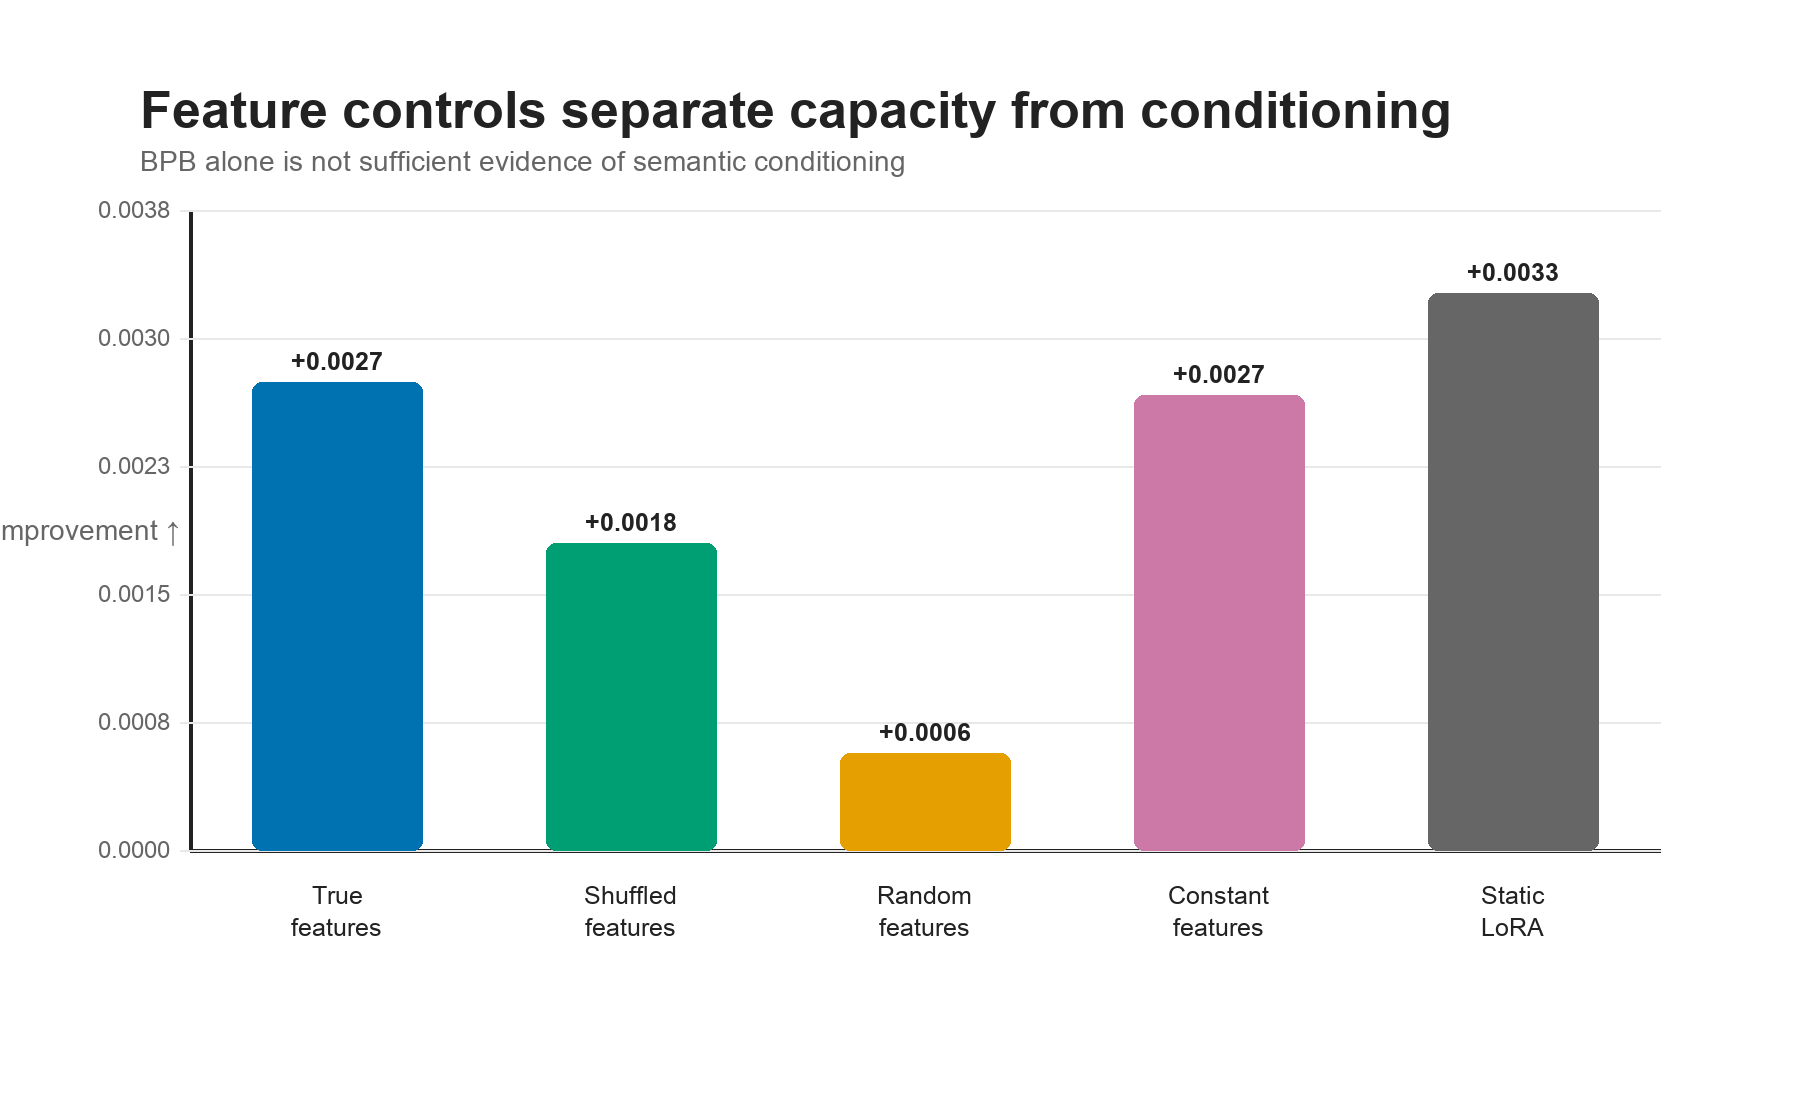
\includegraphics[width=0.82\linewidth]{paper_feature_controls.png}
\caption{Feature controls for the bridge. Shuffled features remove sensor alignment; random features test stochastic conditioning.}
\label{fig:controls}
\end{figure}

\subsection{Composition}
Independently trained bridges can be averaged in LoRA space. Table~\ref{tab:composition} and Figure~\ref{fig:composition} show that composition remains feasible but is not additive: extra modalities can dilute or interfere with each other when merged without a learned router. Composition bricks train for 150 steps each versus 300 for the Table~\ref{tab:main} bridges, so single-modality rows in the two tables are not directly comparable.

\begin{table}[t]
\centering
\caption{Conditioned additive merge of independently trained bridges.}
\label{tab:composition}
\begin{tabular}{lrrrr}
\toprule
Active modalities & Count & Baseline & Final & $\Delta$ BPB \\
\midrule
Vision & 1 & 1.9654 & 1.9633 & +0.0021 \\
Audio & 1 & 1.9654 & 1.9644 & +0.0010 \\
IMU & 1 & 1.9654 & 1.9648 & +0.0006 \\
Vision+Audio & 2 & 1.9654 & 1.9639 & +0.0016 \\
Vision+IMU & 2 & 1.9654 & 1.9636 & +0.0018 \\
Audio+IMU & 2 & 1.9654 & 1.9638 & +0.0016 \\
Vision+Audio+IMU & 3 & 1.9654 & 1.9641 & +0.0013 \\
\bottomrule
\end{tabular}
\end{table}

\begin{figure}[t]
\centering
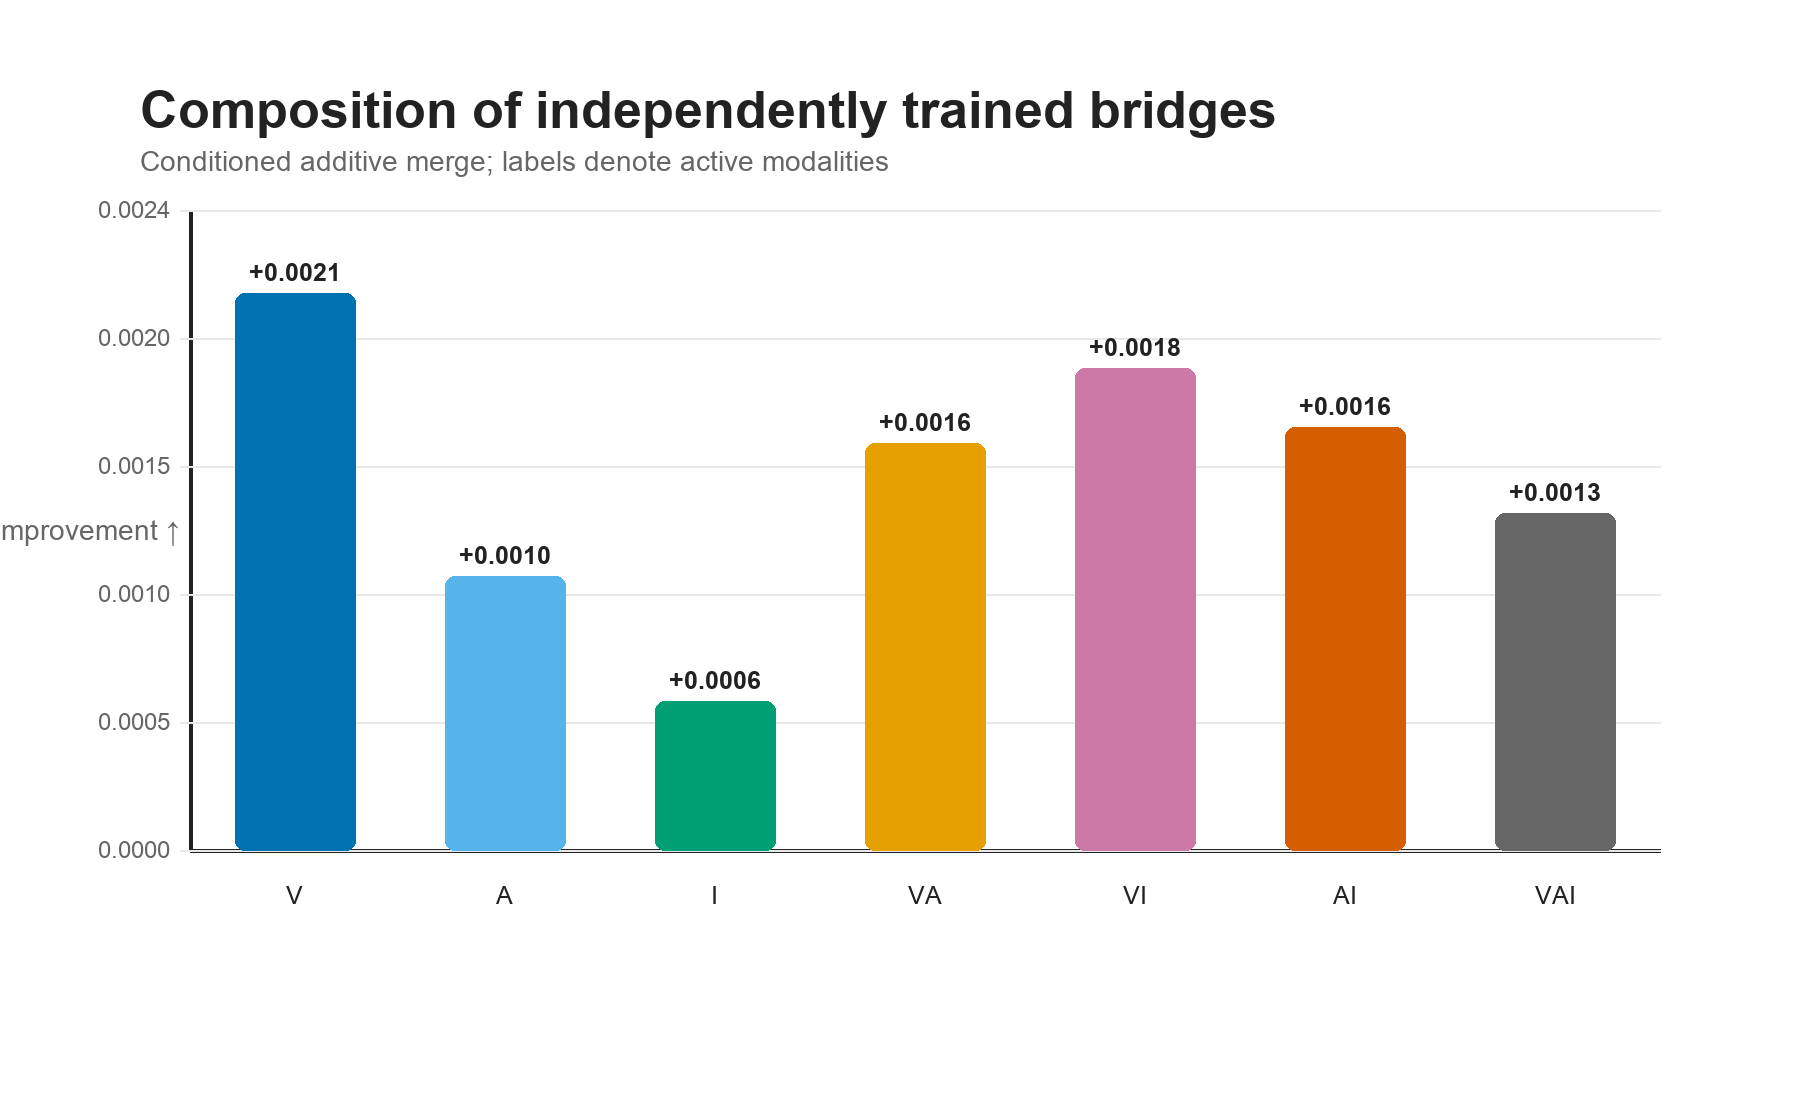
\includegraphics[width=0.82\linewidth]{paper_composition.png}
\caption{Composition of independently trained bridges. Simple averaging exposes interference between low-rank update subspaces.}
\label{fig:composition}
\end{figure}

\subsection{Diversity and weight-space structure}
\label{sec:diversity}
Table~\ref{tab:diversity} and Figure~\ref{fig:diversity} measure the generated-weight collapse directly. With no regularization, cross-input cosine similarity is close to one. Increasing the diversity penalty reduces this collapse and makes generated LoRA weights more input-dependent, although the BPB improvement may trade off against weight-space diversity.

\begin{table}[t]
\centering
\caption{IMU diversity sweep. Cross-input cosine is measured on held-out activity examples; lower cosine means less collapse. Motion/still cosine is the mean cosine between motion-activity and stationary-activity centroid weights; lower values indicate clearer separation of the two clusters.}
\label{tab:diversity}
\begin{tabular}{rrrr}
\toprule
$\lambda$ & $\Delta$ BPB & Cross-input cosine & Motion/still cosine \\
\midrule
0.00 & +0.0026 & 0.9668 & 0.9618 \\
0.01 & +0.0020 & 0.9185 & 0.9277 \\
0.05 & +0.0008 & 0.6471 & 0.6247 \\
0.10 & +0.0009 & 0.4421 & 0.4284 \\
0.20 & +0.0000 & 0.5493 & 0.4530 \\
\bottomrule
\end{tabular}
\end{table}

\begin{figure}[t]
\centering
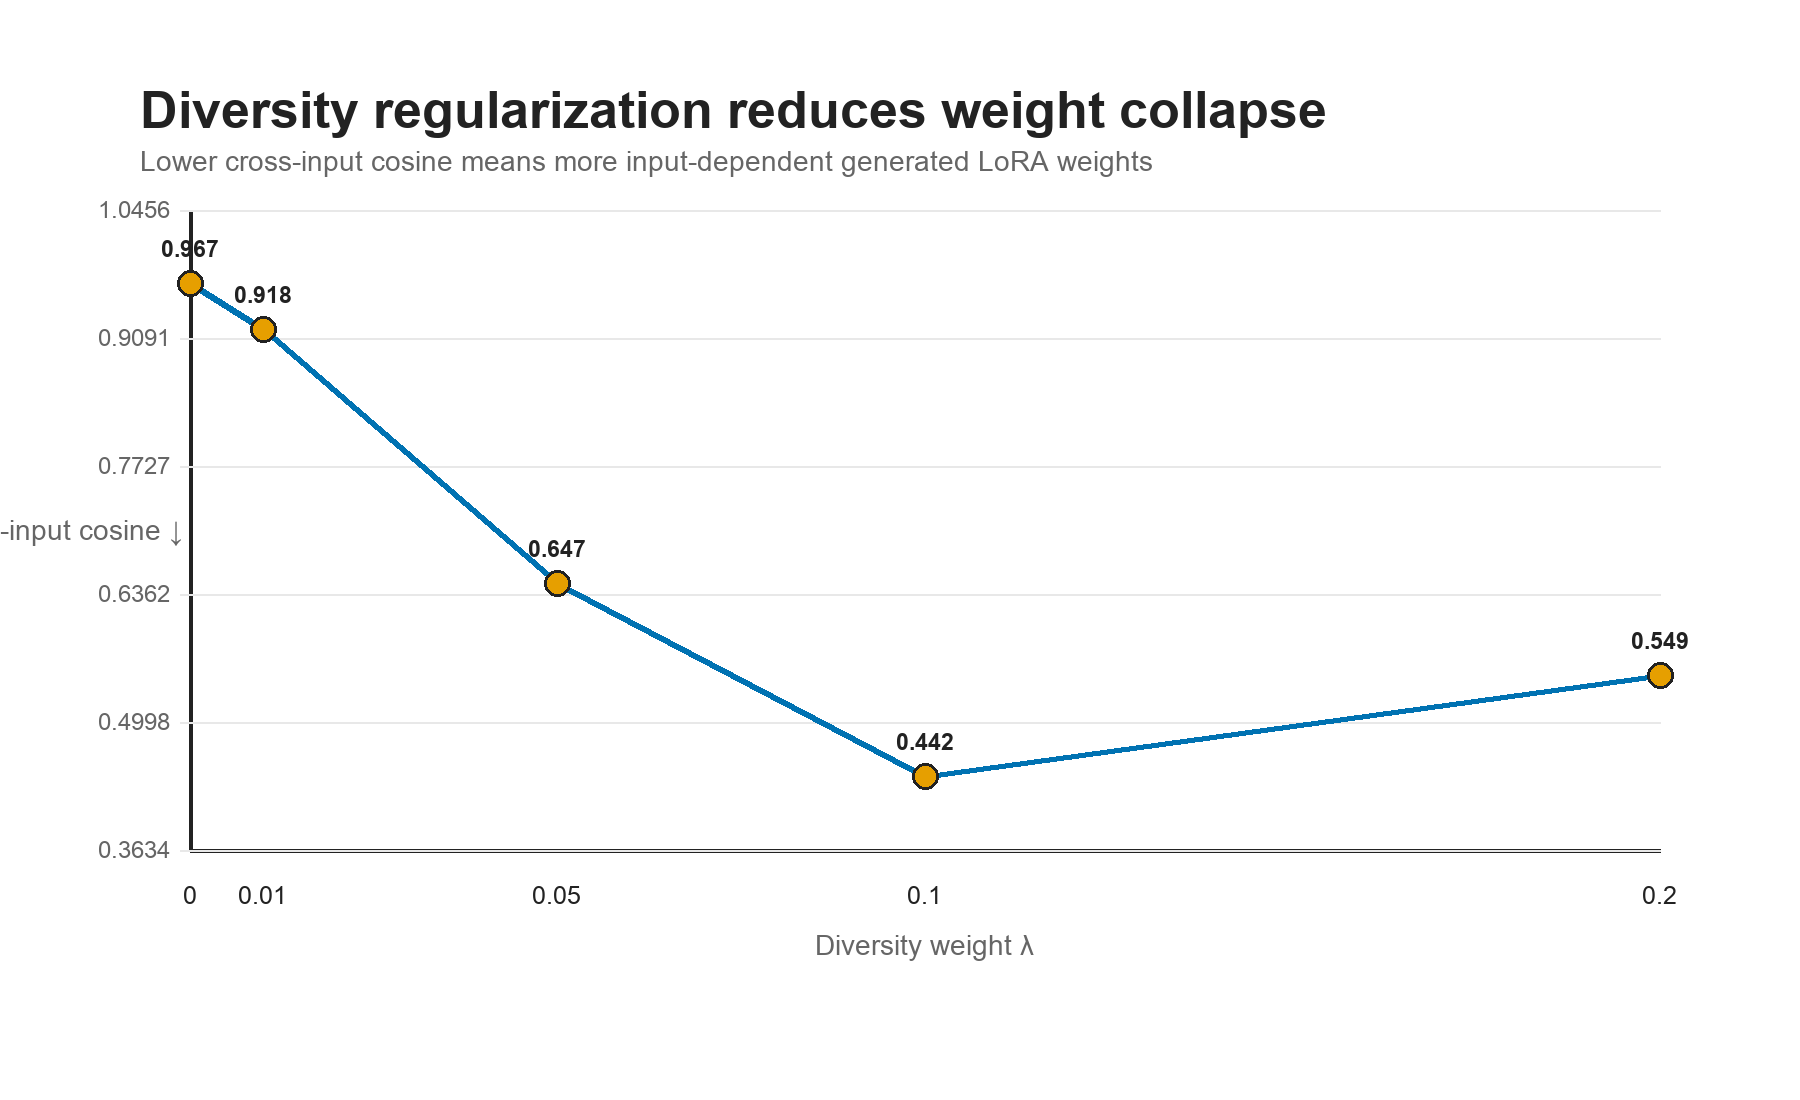
\includegraphics[width=0.82\linewidth]{paper_diversity_ablation.png}
\caption{Diversity regularization reduces generated-weight collapse across IMU inputs.}
\label{fig:diversity}
\end{figure}

\subsection{Task-aligned and reproducibility probes}
Task ranking evaluates whether the adapted model assigns higher likelihood to the correct sensor label in a short text prompt, scored on the natural tokenization of prompt+label over a label-stratified held-out subset; the no-bridge condition applies a zero LoRA and serves as the chance-level reference. Here the conditioning that BPB cannot see is unmistakable (Table~\ref{tab:task}). On six-way IMU activities, true features reach 0.80 rank-1 accuracy and 1.23 average rank, against 0.17 and chance-level ranking for the unconditioned model --- and, critically, for the shuffled and random controls as well. On fifty-way audio events, true features reach 0.33 rank-1 (9.97 average rank) where chance is 0.02 and every control again sits at chance. The same bridges whose BPB gain is pure capacity are, at the task level, decisively input-dependent: the two metrics dissociate cleanly, which is the central methodological point of this paper.

Table~\ref{tab:repro} and Figure~\ref{fig:repro} report three-seed stability for the conditional bridges: with fixed step counts, a repeated run with the same seed reproduces the benchmark value exactly, so the per-seed spread isolates seed sensitivity.

\begin{table}[t]
\centering
\caption{Task-aligned ranking probes. Lower average rank is better; higher rank-1/top-2 is better.}
\label{tab:task}
\begin{tabular}{llrrr}
\toprule
Modality & Condition & Avg. rank & Rank-1 & Top-2 \\
\midrule
Audio & no bridge & 25.28 & 0.03 & 0.05 \\
Audio & true & 9.97 & 0.33 & 0.53 \\
Audio & shuffled & 25.36 & 0.02 & 0.05 \\
Audio & random & 24.92 & 0.03 & 0.06 \\
IMU & no bridge & 3.53 & 0.17 & 0.33 \\
IMU & true & 1.23 & 0.80 & 0.98 \\
IMU & shuffled & 3.50 & 0.16 & 0.31 \\
IMU & random & 3.39 & 0.16 & 0.31 \\
\bottomrule
\end{tabular}
\end{table}

\begin{table}[t]
\centering
\caption{Three-seed stability for conditional bridges (seeds 42, 1042, 2042).}
\label{tab:repro}
\begin{tabular}{lrl}
\toprule
Modality & Mean $\Delta$ BPB & Per-seed $\Delta$ BPB \\
\midrule
Audio & +0.0026 & +0.0025, +0.0027, +0.0026 \\
Vision & +0.0028 & +0.0031, +0.0029, +0.0023 \\
IMU & +0.0027 & +0.0026, +0.0027, +0.0026 \\
\bottomrule
\end{tabular}
\end{table}

\begin{figure}[t]
\centering
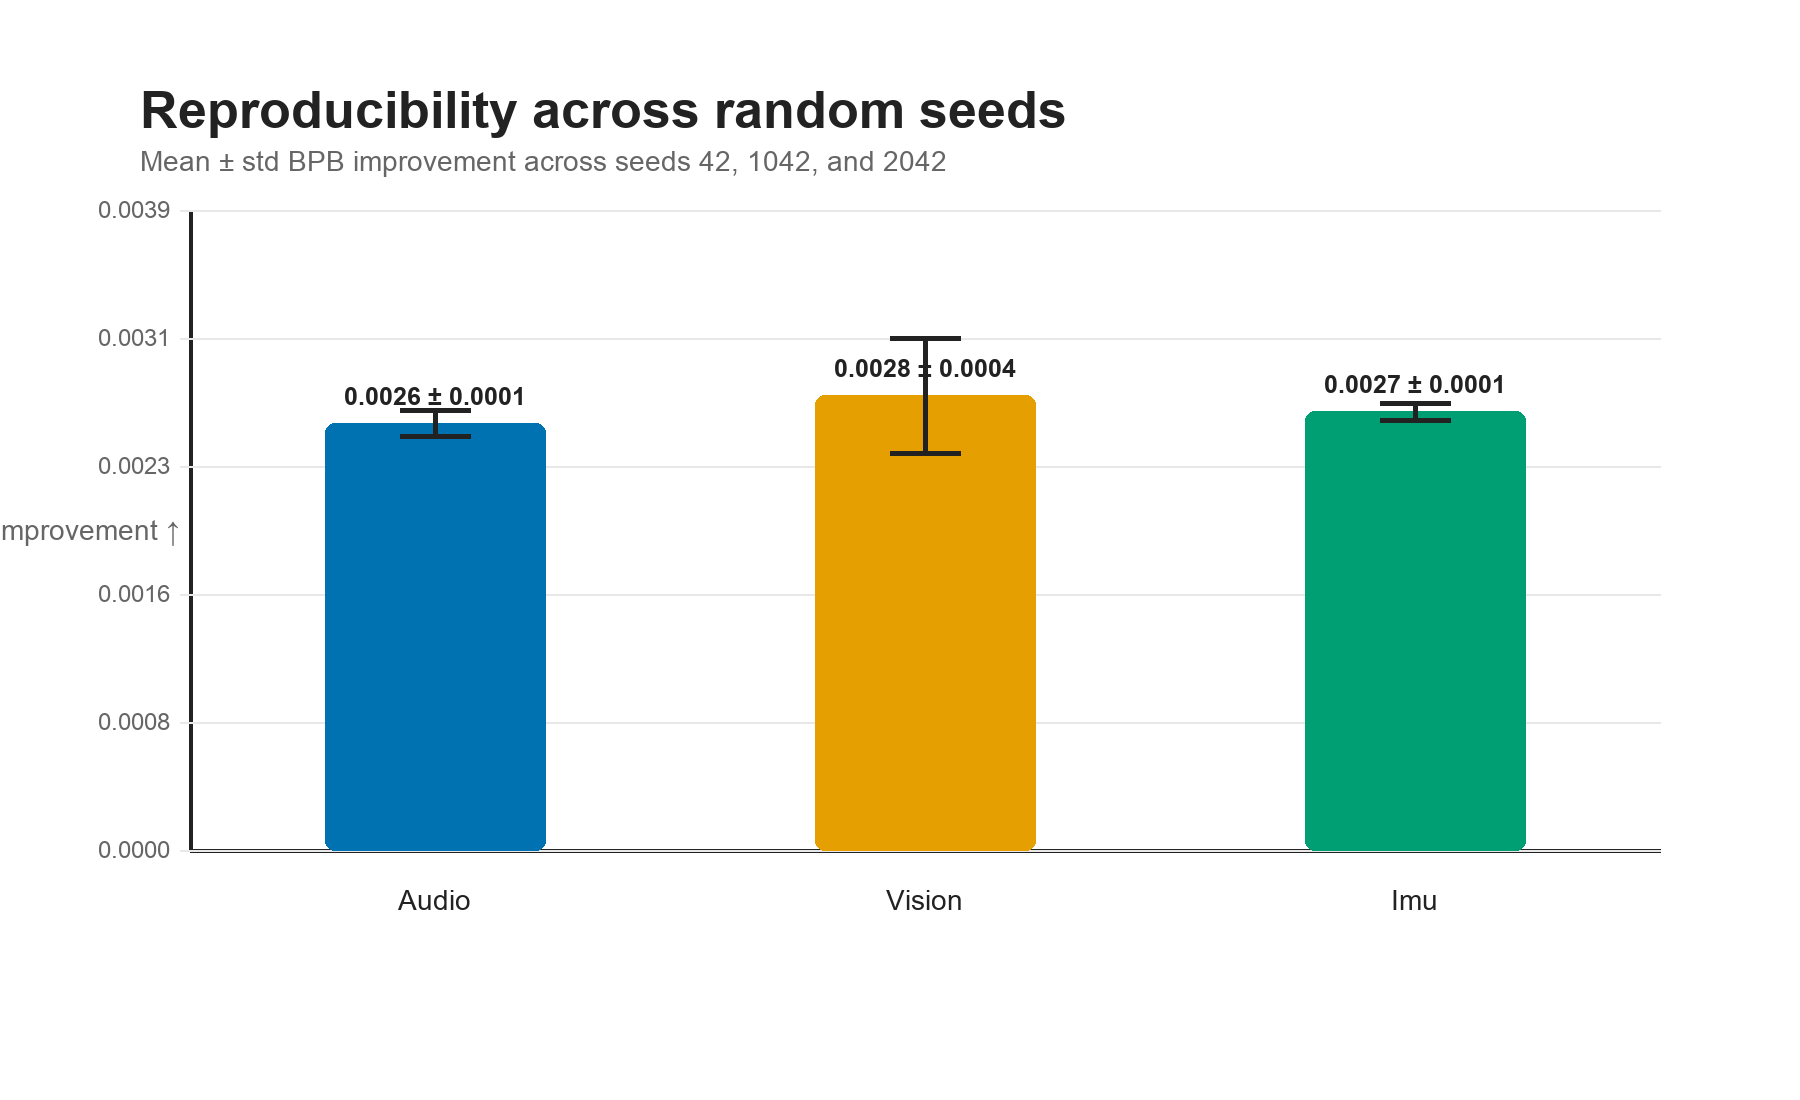
\includegraphics[width=0.82\linewidth]{paper_reproducibility.png}
\caption{Reproducibility of bridge BPB improvements across random seeds.}
\label{fig:repro}
\end{figure}

\subsection{Budget scaling}
\label{sec:scaling}
To test whether the qualitative picture is an artifact of short training, we repeated the full suite at 10$\times$ the step budget (3000 benchmark steps, 6000 task-probe steps) with a 131072-token eval stream. The BPB ordering is preserved as every condition improves: static LoRA +0.0134 (from +0.0033), conditional bridge +0.0121 (from +0.0027), constant features +0.0120, shuffled +0.0118, random +0.0108; the conditioning contribution measured by BPB remains indistinguishable from zero. Prefix tuning's degradation shrinks toward neutrality (-0.0048 to -0.0016) without ever helping.

The task probes expose a boundary that short budgets hide. The audio probe strengthens with optimization (rank-1 0.33 to 0.36, controls still at chance), but the IMU probe collapses: at 6000 steps the true-feature bridge becomes behaviorally indistinguishable from the zero-LoRA condition (rank-1 0.17, equal to no-bridge), having scored 0.80 at 600 steps. The diversity sweep at this budget shows the same mechanism: $\lambda=0.01$ no longer prevents weight collapse (cross-input cosine 0.99) while $\lambda \ge 0.05$ still does (0.31). Prolonged unregularized training drives the hypernetwork toward input-independent output, and the collapse threshold moves with optimization length --- the failure mode this paper documents is not confined to a corner of the BPB table.

\section{Related Work}
LoRA \cite{hu2021lora} and adapter methods \cite{houlsby2019adapters} adapt frozen transformers \cite{vaswani2017attention} with a small number of trainable parameters. Prefix tuning \cite{li2021prefixtuning} adapts models by prepending continuous tokens; in our experiments token-space conditioning only degrades a frozen small model trained without prefixes. Hypernetworks \cite{ha2016hypernetworks} generate weights for another network; shared hypernetwork adapters \cite{mahabadi2021hyperformer} apply the idea to multi-task adaptation, and HyperTuning \cite{phang2022hypertuning} generates parameter-efficient adaptations from task descriptions with a frozen base model. Our setting differs in that the conditioning signal is a continuous sensor stream rather than a task identifier or instruction text, and the generated weights change per input at evaluation time. Composing the resulting adaptations connects to weight-space model editing and merging \cite{ilharco2023task}, where interference between added task vectors is a known obstacle --- consistent with the sub-additive composition we observe. Multimodal systems such as Flamingo \cite{alayrac2022flamingo} and LLaVA \cite{liu2023llava} integrate external modalities through architectures and training recipes designed for paired data; conditional LoRA bridges instead test a modular interface in which independently trained sensor encoders condition a frozen language model through generated low-rank weight updates. Sensor data come from ESC-50 \cite{piczak2015esc} and UCI-HAR \cite{anguita2013uci}.

\section{Limitations}
The bridge is large relative to the base model (84.3M trainable parameters generating a 327,680-dimensional LoRA vector for a 33.6M-parameter LM), so bridge compression is a central requirement for scaling this interface, not a footnote. All results are on one small base model trained on one corpus; the mechanism findings (capacity/conditioning dissociation, collapse, prefix degradation) are the claims we expect to transfer, not the specific deltas. The task probes use a single prompt template per modality and modest eval subsets. The budget-scaling run shows that probe outcomes can depend strongly on training length, so conclusions drawn at any single budget --- including ours --- should be read against that section. Composition of independently trained bridges remains sub-additive, and we do not yet offer a fix.

\section{Conclusion}
Conditional LoRA bridges connect frozen sensor encoders to frozen language models through generated low-rank weight updates. Our controlled study yields one sharp methodological result and one mechanism result. Methodologically, aggregate language-modeling metrics cannot detect sensor conditioning: a capacity-matched constant-feature control reproduces the bridge's entire BPB gain, while task-aligned probes show decisive input-dependence under exactly the same training. Mechanistically, hypernetwork collapse is the failure mode that governs whether conditioning exists at all: diversity regularization creates input-dependent weight structure, and prolonged unregularized training destroys it along with the task-level conditioning it supports. Weight-space modulation does no harm where token-space injection degrades the frozen model. Future work should compress the bridge (the interface's scaling bottleneck), make composition constructive rather than interfering, and extend the probe suite beyond single-template ranking.

\section*{Reproducibility Statement}
The paper artifacts are generated from a single summary JSON emitted by the repository runner. The exact command that produced the bundled artifact, reconstructed from its recorded metadata, is:
\begin{verbatim}
paper-reproduce --suite all --include-audio-task --benchmark-steps 300 --composition-steps-per-brick 150 --task-steps 600 --eval-tokens 32768 --sensor-limit 64 --max-eval-items 64 --seed 42 --output-dir results/<run>
\end{verbatim}
Training loops run fixed step counts, so a repeated run with the same seed reproduces each number exactly on the same hardware class; absolute BPB values shift by roughly $\pm 0.02$ under a different eval sample, while all reported deltas are paired comparisons on one fixed eval stream shared by every condition.
Figures and manuscript source are regenerated from that run artifact with:
\begin{verbatim}
paper-figures results/<run>/summary.json --output-dir figures
paper-render-arxiv results/<run>/summary.json --output-dir arxiv
\end{verbatim}
Code, checkpoints, data, and the exact result artifacts are available at \url{https://github.com/kortexa-ai/legolm.paper}. The arXiv source package includes this manuscript's result artifacts under \texttt{anc/}; tables, figures, and every number in the text are rendered from them. The runner validates that Git LFS checkpoints are materialized before loading.

\bibliographystyle{plain}
\bibliography{references}
\end{document}
